% !Mode:: "TeX:UTF-8"

\chapter{绪论}
\section{研究背景与意义}
\subsection{研究背景}

在博士学位论文中，研究背景通常采用分段方式逐层展开，从宏观领域到具体研究问题，逻辑上逐步收敛。一般可以分为 3–4 个自然段进行描述，每一段承担不同的功能。

首先介绍研究领域的发展趋势和研究意义，从宏观层面说明该研究方向的重要性。该段应当突出研究领域的应用价值或学术价值，使读者了解研究问题所处的大背景。如：随着人工智能与计算机视觉技术的快速发展，智能感知与行为理解逐渐成为计算机视觉领域的重要研究方向。人体动作分析作为其中的关键任务，在智能监控、人机交互、虚拟现实以及医疗康复等领域具有广泛应用价值。通过对人体动作的准确建模与理解，能够有效提升智能系统对复杂场景的感知能力，因此受到了学术界和工业界的广泛关注。

在宏观背景基础上，进一步聚焦到具体研究对象或研究任务，并说明其研究特点或优势。如：在人体行为理解研究中，基于骨骼数据的动作表示由于能够直接反映人体关节的空间结构信息，同时对外观变化和背景干扰具有较强鲁棒性，近年来逐渐成为研究热点。与传统基于RGB视频的方法相比，骨骼数据具有结构清晰、维度较低等特点，使其更适合进行人体动作的时空建模。然而，骨骼动作序列通常包含复杂的空间拓扑关系和时间动态变化，如何有效建模其时空依赖关系仍然是一个具有挑战性的研究问题。

进一步介绍目前主流研究方法，并指出其存在的不足，从而引出研究问题。如：现有研究主要采用卷积神经网络、图卷积网络以及Transformer等深度学习模型对骨骼动作进行建模。其中，图卷积网络能够利用人体骨骼的拓扑结构信息，在动作识别任务中取得了较好的效果。然而，这类方法在建模长程时空依赖关系以及复杂动作动态变化方面仍存在一定局限。此外，在动作生成任务中，传统生成模型在生成稳定性和动作真实性方面仍面临挑战。因此，探索更加有效的人体动作建模与生成方法仍具有重要研究意义。

\subsection{研究意义}

研究意义主要用于说明本研究开展的价值与贡献，通常从 理论意义 和 实际应用意义 两个方面进行阐述。通过研究意义的描述，可以进一步突出论文研究工作的必要性和重要性。

随着移动互联网以及人工智能的发展，人类社会已经进入了数字化、信息化和智能化的时代。而计算机视觉技术作为分析和处理海量数据的关键技术，已在深度学习领域发挥出了巨大效用。人是大量视觉数据的主要目标，人体行为是实现目的、欲望、意识和意志等的主要手段，是人的一种重要的社会属性，如图\ref{fig:applications}所示。

\begin{figure}[htbp]
    \centering
    \begin{subfigure}[b]{0.4\textwidth}
        \centering
          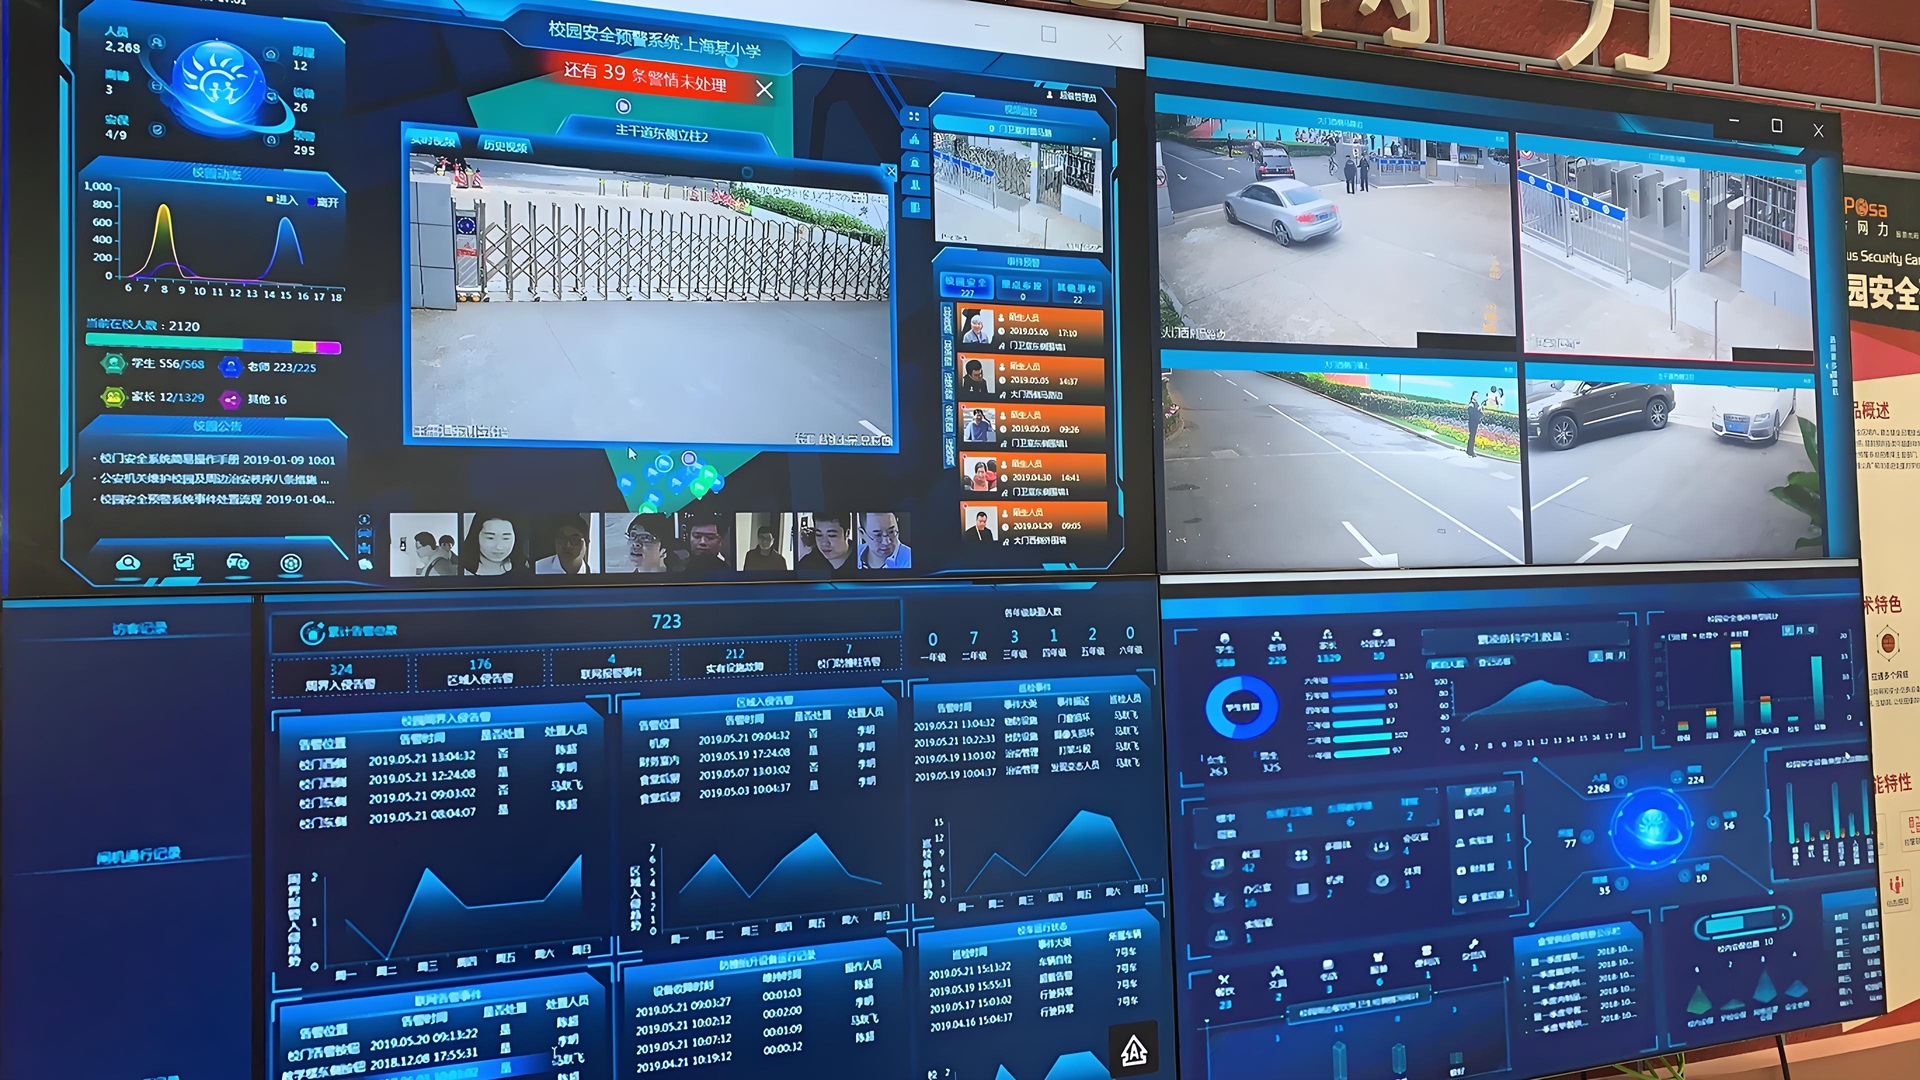
\includegraphics[width=\linewidth]{figures/Fig1a.jpg}
        \caption{安防监控}
    \end{subfigure}
    \hspace*{15pt}
    \begin{subfigure}[b]{0.4\textwidth}
        \centering
        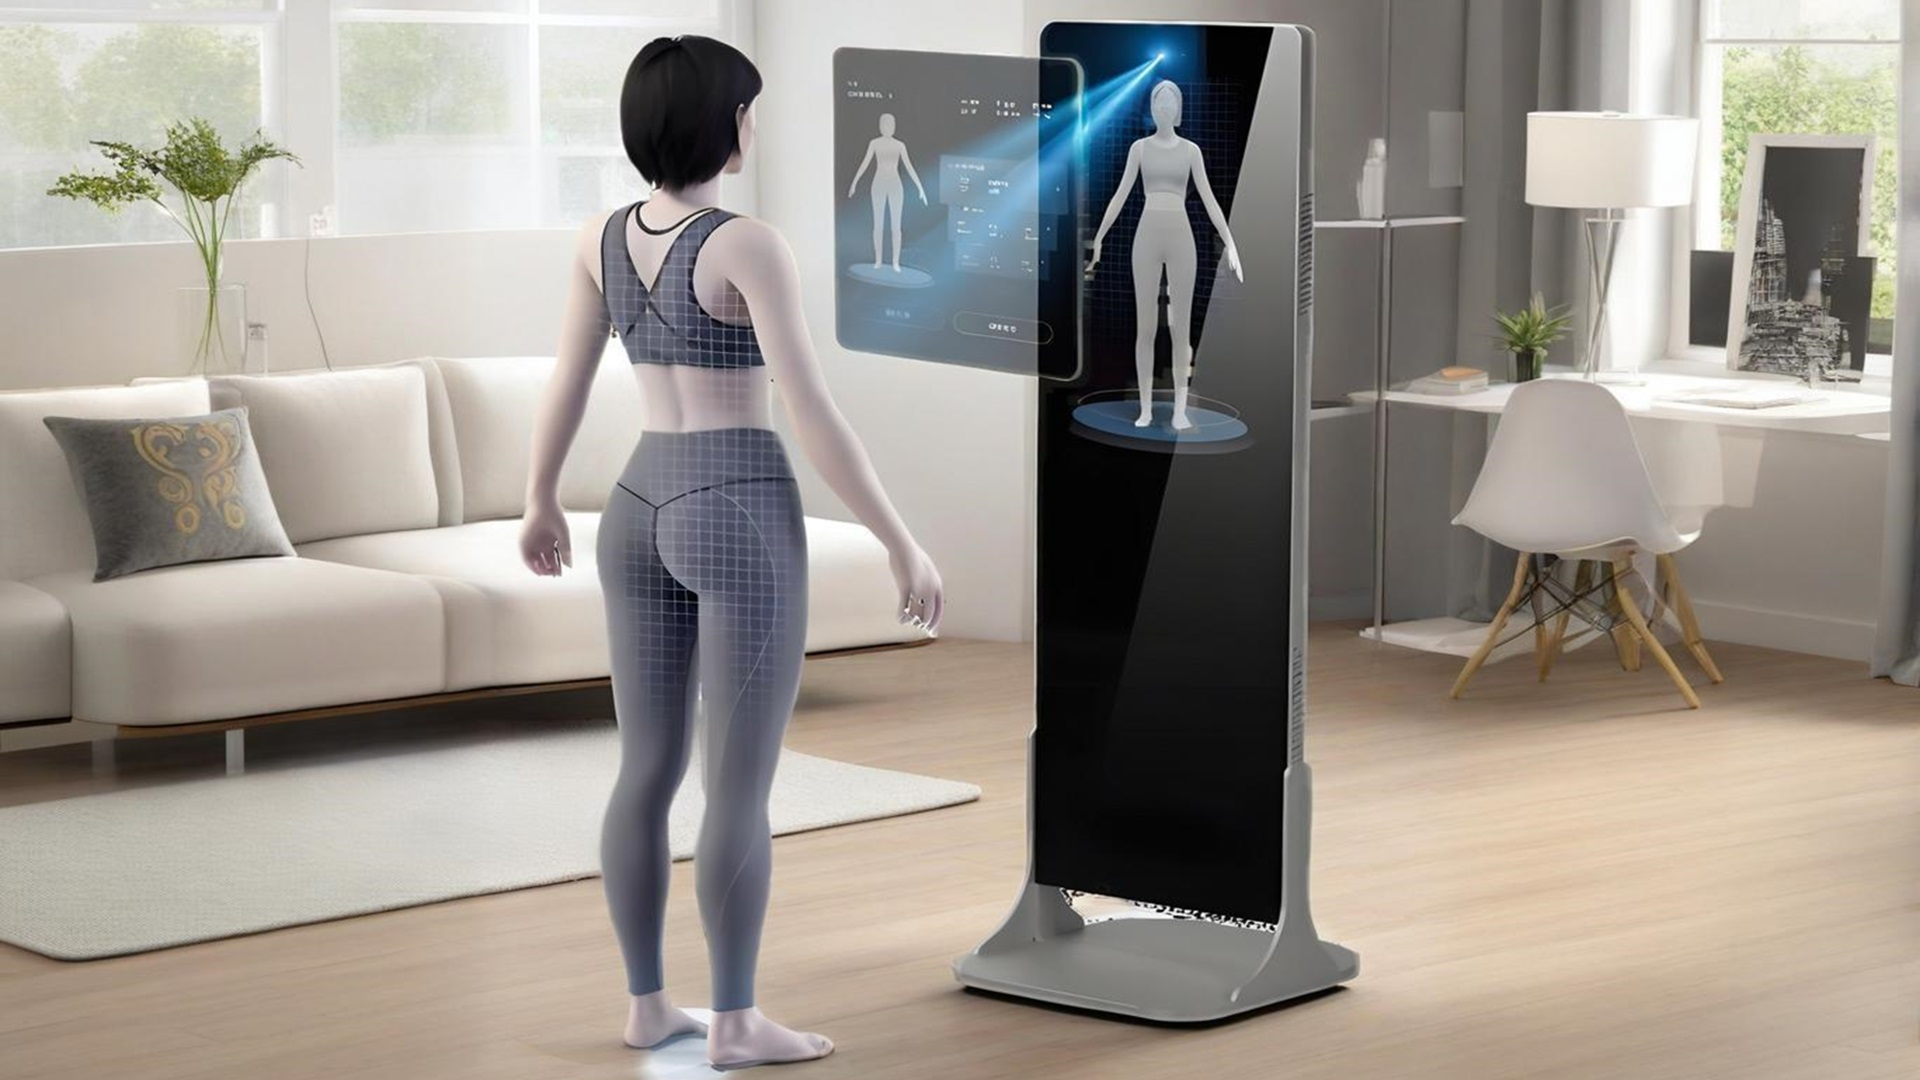
\includegraphics[width=\linewidth]{figures/Fig1b.jpg}
        \caption{智能家居}
    \end{subfigure}
    \\
    \begin{subfigure}[b]{0.4\textwidth}
        \centering
        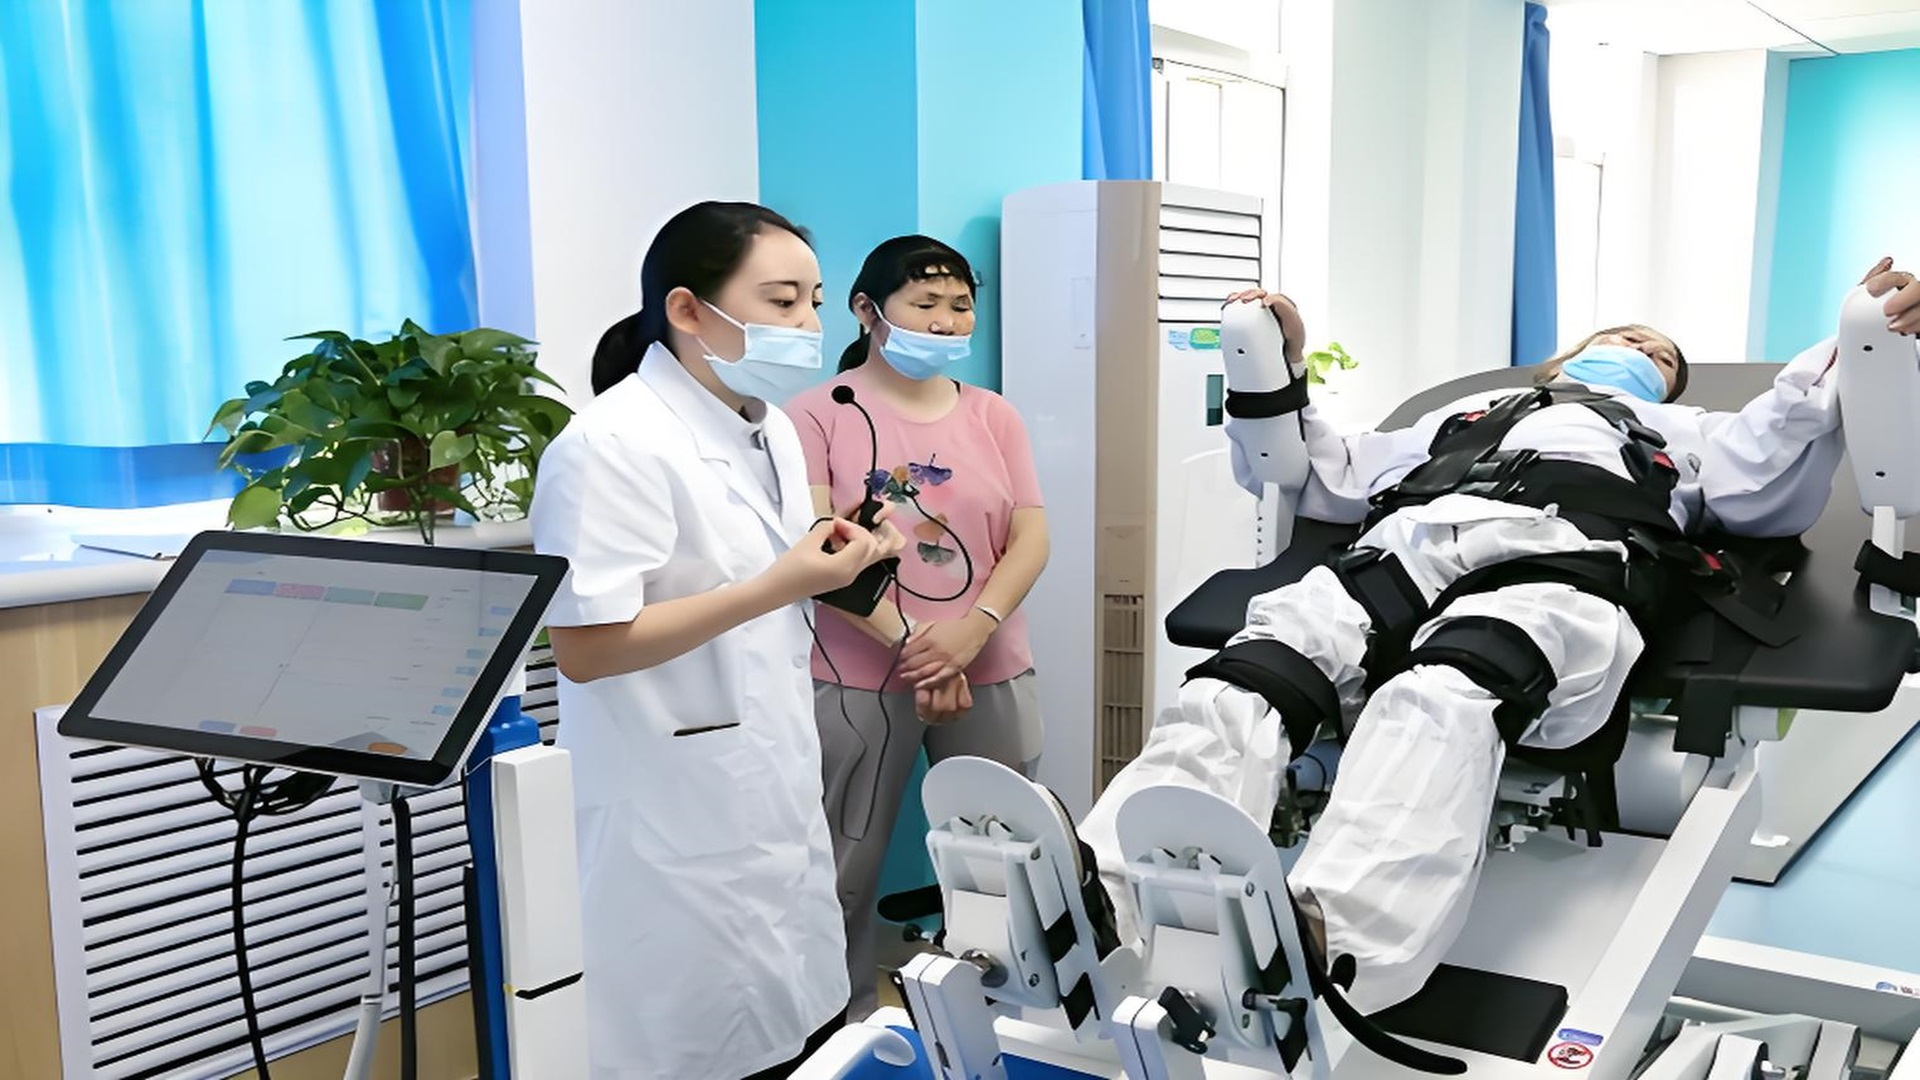
\includegraphics[width=\linewidth]{figures/Fig1c.jpg}
        \caption{医疗康复}
    \end{subfigure}
    \hspace*{15pt}
    \begin{subfigure}[b]{0.4\textwidth}
        \centering
        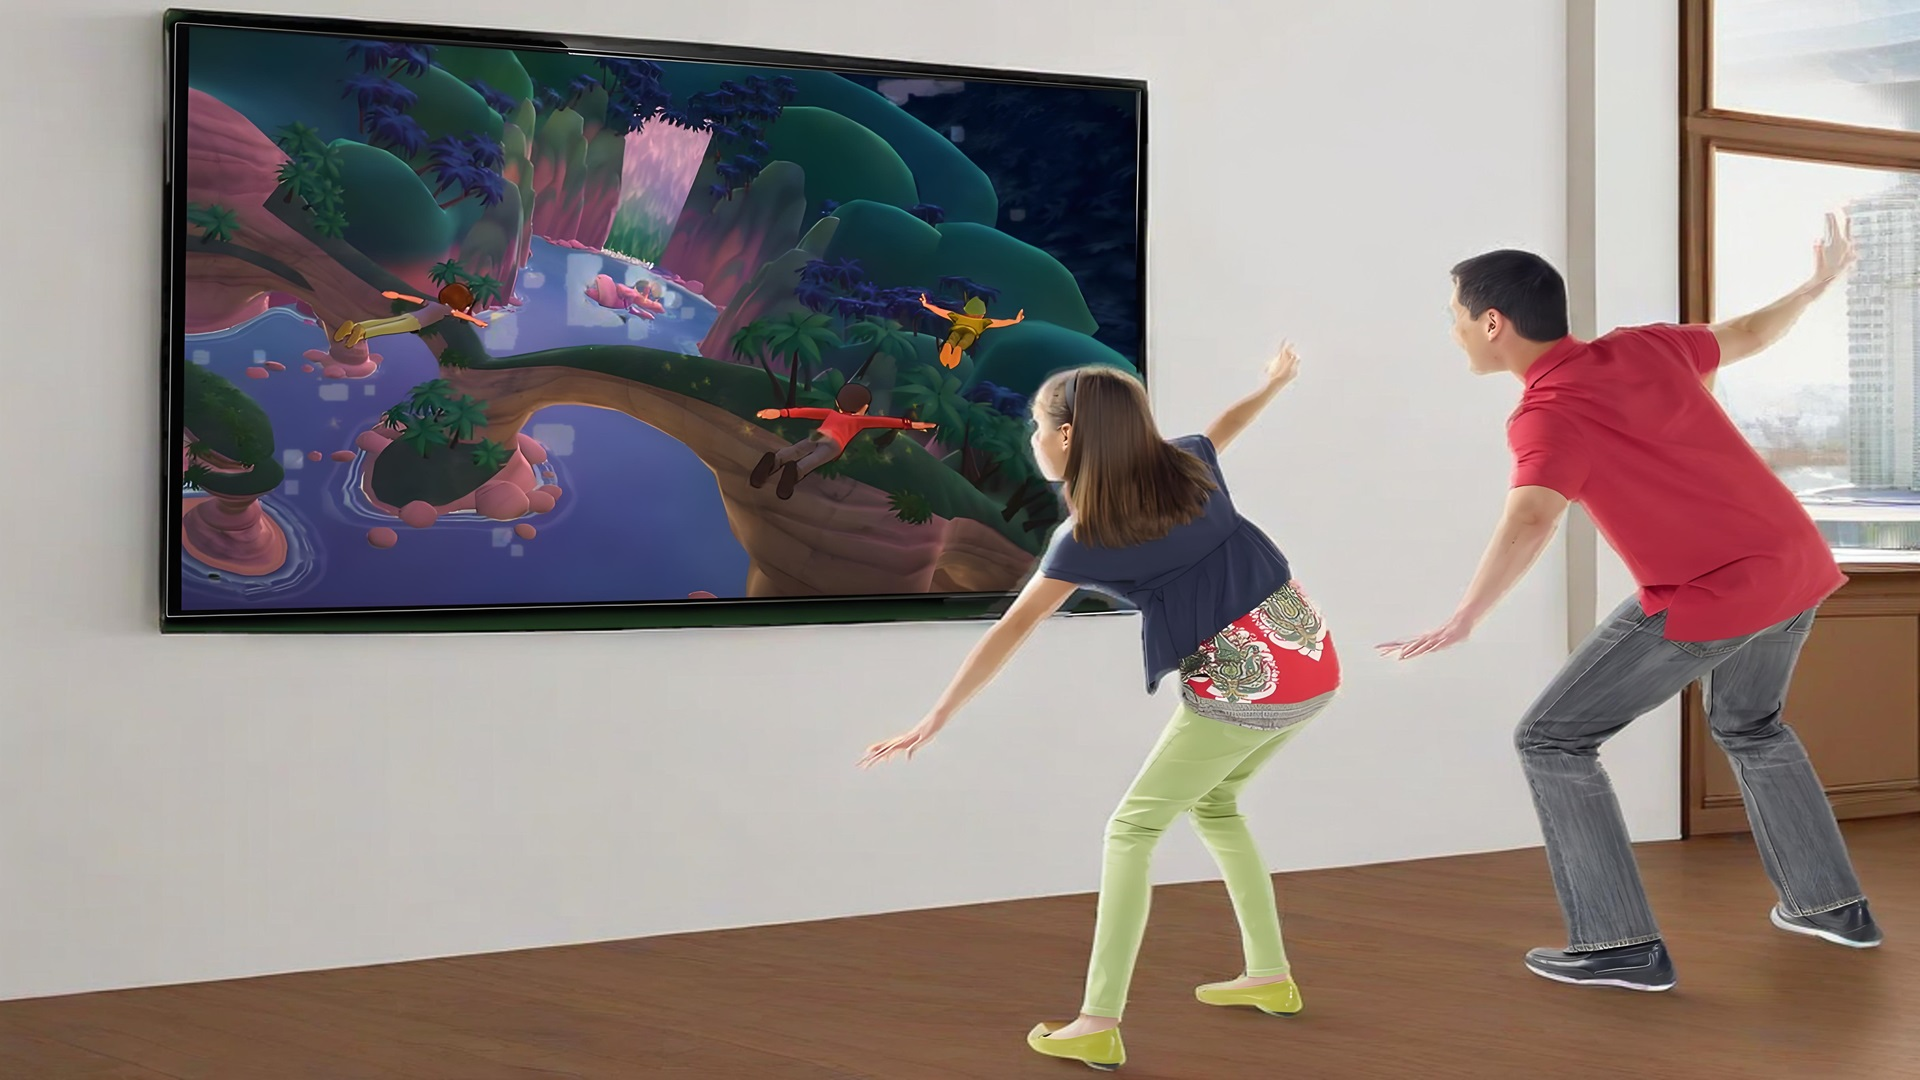
\includegraphics[width=\linewidth]{figures/Fig1d.jpg}
        \caption{人机交互}
    \end{subfigure}
\bilingualfigure{人体行为分析应用领域}{Applications of human action Analysis}
\label{fig:applications}
\end{figure}

\section{国内外研究现状}

在博士论文绪论中，“国内外研究现状”部分主要用于系统梳理该领域已有研究成果，并指出现有研究的不足，从而为论文研究内容提供依据。该部分通常采用分段或分小节的方式进行论述，按照研究方向或技术路线进行分类介绍，而不是简单罗列文献。

\subsection{XXX国内外现状}

\subsection{XXX国内外现状}

\subsection{XXX国内外现状}

\section{拟解决的关键问题}

在博士学位论文绪论中，“拟解决的关键问题”部分主要用于明确论文研究所要突破的核心问题，是从前面的研究现状与不足自然过渡而来的。该部分通常不需要很长，但需要概括准确、逻辑清晰、突出问题本质。一般可先用一段总体说明，然后以条目式或分段方式列出若干关键问题。

\section{本文研究内容}

在博士论文绪论中，“本文研究内容”部分主要用于概括论文开展的具体研究工作。该部分通常在“拟解决的关键问题”之后，通过条目式或分段方式介绍论文的主要研究内容，使读者能够清晰了解论文各项研究工作的整体结构。一般先给出一段总体说明，然后列出 3–5 项具体研究内容。

\section{本文组织结构}

在博士学位论文绪论中，“本文组织结构”部分主要用于介绍论文各章节的安排，使读者能够快速了解论文整体结构与内容分布。该部分通常采用一段总述 + 分章节说明的写法，对每一章的主要内容进行简要概括。